\documentclass{article}
\usepackage{color}
\usepackage{tikz}

\definecolor{kclass0}{HTML}{960000}
\definecolor{kclass1}{HTML}{FF0000}
\definecolor{kclass2}{HTML}{FF6E6E}
\definecolor{kclass3}{HTML}{FFCCCC}
\definecolor{kclass4}{HTML}{CC8D14}
\definecolor{kclass5}{HTML}{CCAA54}
\definecolor{kclass6}{HTML}{FFCC00}
\definecolor{kclass7}{HTML}{FFFF64}
\definecolor{kclass8}{HTML}{007800}
\definecolor{kclass9}{HTML}{005000}
\definecolor{kclass10}{HTML}{003200}
\definecolor{kclass11}{HTML}{96FF00}
\definecolor{kclass12}{HTML}{00D700}
\definecolor{kclass13}{HTML}{BEBE00}
\definecolor{kclass14}{HTML}{8C8C00}
\definecolor{kclass15}{HTML}{5A5A00}
\definecolor{kclass16}{HTML}{550055}
\definecolor{kclass17}{HTML}{820082}
\definecolor{kclass18}{HTML}{C800C8}
\definecolor{kclass19}{HTML}{FF6EFF}
\definecolor{kclass20}{HTML}{646464}
\definecolor{kclass21}{HTML}{8C8C8C}
\definecolor{kclass22}{HTML}{BEBEBE}
\definecolor{kclass23}{HTML}{6E28B4}
\definecolor{kclass24}{HTML}{B464FA}
\definecolor{kclass25}{HTML}{C89BFA}
\definecolor{kclass26}{HTML}{C8C8FF}
\definecolor{kclass27}{HTML}{64FFFF}

\newcommand{\bplotHist}[3]{
\node[anchor=west] at (-8., -#2) {#1};
\foreach \b/\w/\c in {#3}{ %0.00/21.72/kclass0,21.72/18.96/kclass1,40.68/2.71/kclass2}{
\draw [color=white,fill=\c, fill opacity=.8, line width=.1pt] (\b,{-#2-.45}) rectangle +(\w,.9);
}
}
\newcommand{\bplotHistV}[3]{
\node[anchor=west] at (-5.8, -#2) {\small{#1}};
\foreach \b/\w/\c in {#3}{ %0.00/21.72/kclass0,21.72/18.96/kclass1,40.68/2.71/kclass2}{
\draw [color=white,fill=\c, fill opacity=.8, line width=.1pt] (\b,{-#2-.225}) rectangle +(\w,.45);
}
}
\newcommand{\bplotHistL}[3]{
\foreach \b/\w/\c in {#3}{ %0.00/21.72/kclass0,21.72/18.96/kclass1,40.68/2.71/kclass2}{
\draw [color=white,fill=\c, fill opacity=.8, line width=.1pt] (\b,{-#2-.5}) rectangle +(\w,.225);
}
}

\begin{document}
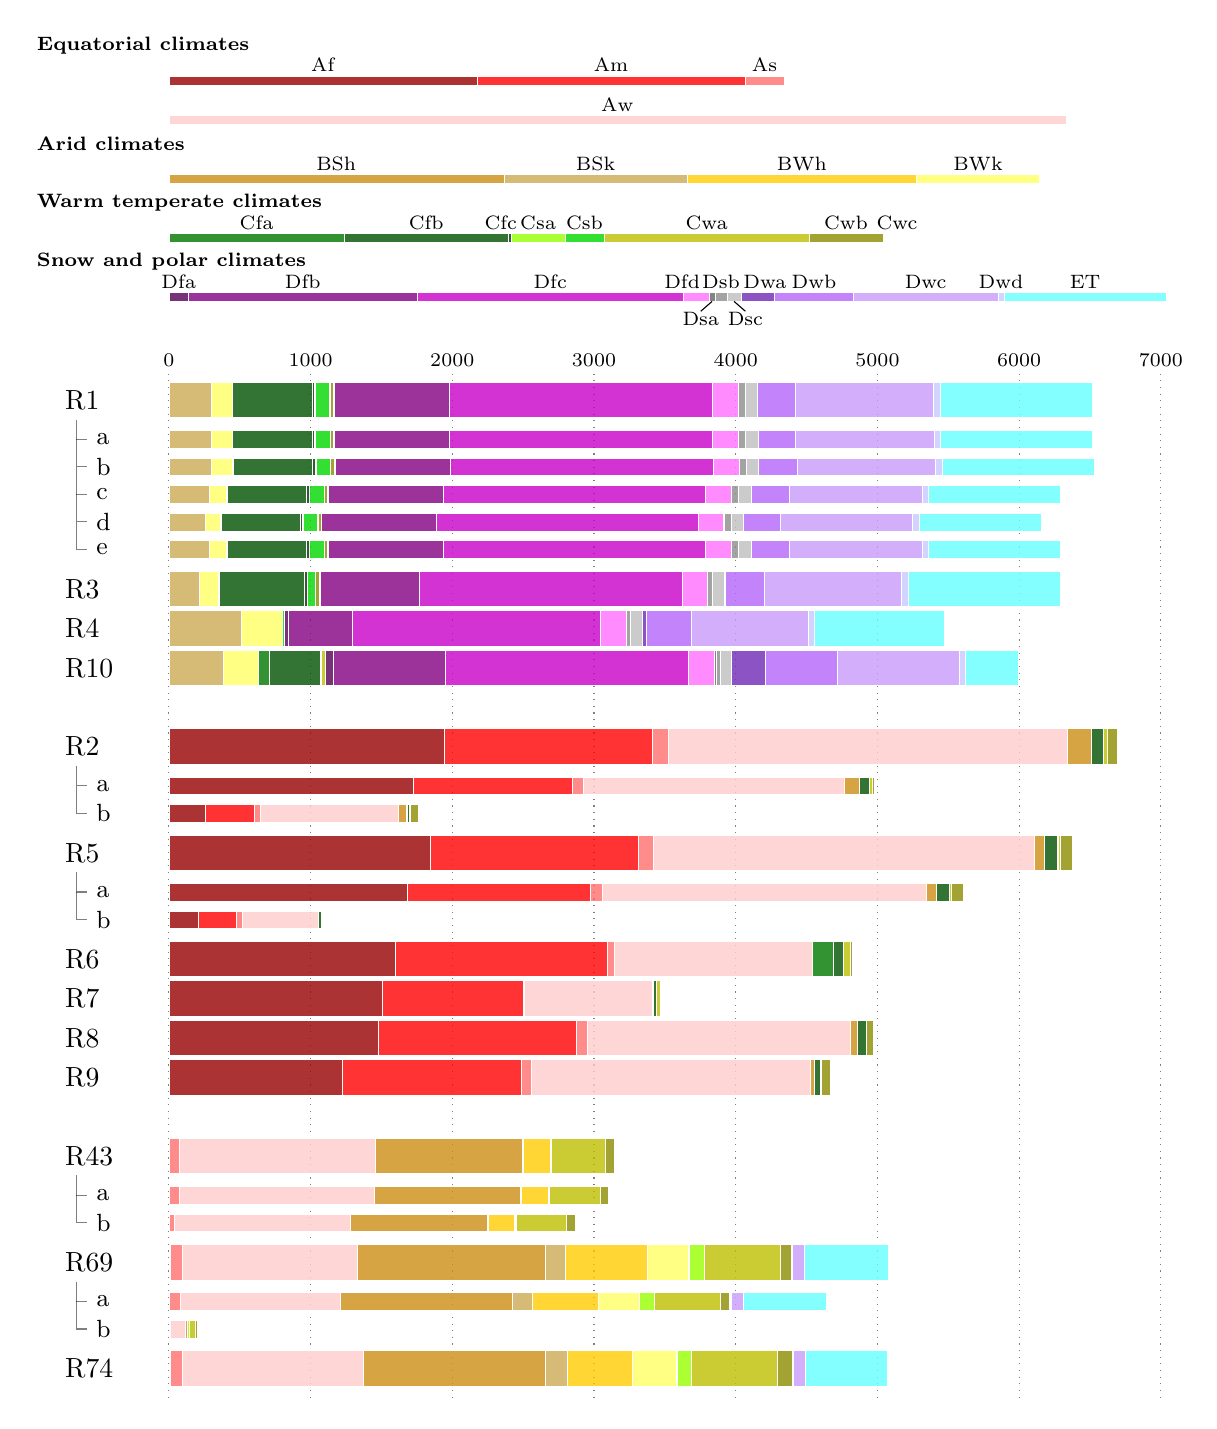
\begin{tikzpicture}[xscale=.18, yscale=0.5]
%% \draw[opacity=0.5, dotted] (0,5.8) -- (0,-26.4);
\draw[opacity=0.5, dotted] (0,0) -- (0,-26.4);
\node[anchor=center, fill=white, inner sep=2pt] at (0, 0) {\scriptsize{$0$}};
\draw[opacity=0.5, dotted] (10,0) -- (10,-26.4);
\node[anchor=center, fill=white, inner sep=2pt] at (10, 0) {\scriptsize{$1000$}};
\draw[opacity=0.5, dotted] (20,0) -- (20,-26.4);
\node[anchor=center, fill=white, inner sep=2pt] at (20, 0) {\scriptsize{$2000$}};
\draw[opacity=0.5, dotted] (30,0) -- (30,-26.4);
\node[anchor=center, fill=white, inner sep=2pt] at (30, 0) {\scriptsize{$3000$}};
\draw[opacity=0.5, dotted] (40,0) -- (40,-26.4);
\node[anchor=center, fill=white, inner sep=2pt] at (40, 0) {\scriptsize{$4000$}};
\draw[opacity=0.5, dotted] (50,0) -- (50,-26.4);
\node[anchor=center, fill=white, inner sep=2pt] at (50, 0) {\scriptsize{$5000$}};
\draw[opacity=0.5, dotted] (60,0) -- (60,-26.4);
\node[anchor=center, fill=white, inner sep=2pt] at (60, 0) {\scriptsize{$6000$}};
\draw[opacity=0.5, dotted] (70,0) -- (70,-26.4);
\node[anchor=center, fill=white, inner sep=2pt] at (70, 0) {\scriptsize{$7000$}};



\bplotHistL{A*}{-7.5}{0.00/21.72/kclass0,21.72/18.96/kclass1,40.68/2.71/kclass2}
\bplotHistL{Aw}{-6.5}{0.00/63.28/kclass3}
\bplotHistL{B*}{-5}{0.00/23.63/kclass4,23.63/12.97/kclass5,36.60/16.14/kclass6,52.74/8.70/kclass7}
\bplotHistL{C*}{-3.5}{0.00/12.38/kclass8,12.38/11.55/kclass9,23.93/0.19/kclass10,24.12/3.85/kclass11,27.97/2.72/kclass12,30.69/14.50/kclass13,45.19/5.18/kclass14,50.37/0.03/kclass15}
\bplotHistL{DE}{-2}{0.00/1.38/kclass16,1.38/16.14/kclass17,17.52/18.79/kclass18,36.31/1.81/kclass19,38.12/0.42/kclass20,38.54/0.85/kclass21,39.39/0.97/kclass22,40.36/2.37/kclass23,42.73/5.58/kclass24,48.31/10.18/kclass25,58.49/0.46/kclass26,58.95/11.40/kclass27}
% \bplotHistL{D}{-2}{0.00/1.38/kclass16,1.38/16.14/kclass17,17.52/18.79/kclass18,36.31/1.81/kclass19,38.12/0.42/kclass20,38.54/0.85/kclass21,39.39/0.97/kclass22,40.36/2.37/kclass23,42.73/5.58/kclass24,48.31/10.18/kclass25,58.49/0.46/kclass26}
% \bplotHistL{E}{-1}{0.00/11.40/kclass27}

%%%%%%% GROUP 1
\bplotHist{R1}{1}{0.00/2.99/kclass5,2.99/1.45/kclass7,4.44/0.05/kclass8,4.49/5.60/kclass9,10.09/0.18/kclass10,10.27/0.05/kclass11,10.32/1.02/kclass12,11.34/0.01/kclass13,11.35/0.26/kclass14,11.61/0.01/kclass15,11.62/0.03/kclass16,11.65/8.10/kclass17,19.75/18.58/kclass18,38.33/1.81/kclass19,40.14/0.02/kclass20,40.16/0.48/kclass21,40.64/0.90/kclass22,41.54/2.66/kclass24,44.20/9.76/kclass25,53.96/0.46/kclass26,54.42/10.75/kclass27}

\draw[opacity=0.5] (-6.5,-1.5) -- (-6.5,-2) -- (-5.8,-2);
\draw[opacity=0.5] (-6.5,-2) -- (-6.5,-2.7) -- (-5.8,-2.7);
\draw[opacity=0.5] (-6.5,-2.7) -- (-6.5,-3.4) -- (-5.8,-3.4);
\draw[opacity=0.5] (-6.5,-3.4) -- (-6.5,-4.1) -- (-5.8,-4.1);
\draw[opacity=0.5] (-6.5,-4.1) -- (-6.5,-4.8) -- (-5.8,-4.8);

\bplotHistV{a}{2}{0.00/3.00/kclass5,3.00/1.45/kclass7,4.45/0.05/kclass8,4.50/5.60/kclass9,10.10/0.18/kclass10,10.28/0.05/kclass11,10.33/1.02/kclass12,11.35/0.01/kclass13,11.36/0.26/kclass14,11.62/0.01/kclass15,11.63/0.03/kclass16,11.66/8.10/kclass17,19.76/18.58/kclass18,38.34/1.81/kclass19,40.15/0.02/kclass20,40.17/0.48/kclass21,40.65/0.90/kclass22,41.55/2.66/kclass24,44.21/9.76/kclass25,53.97/0.46/kclass26,54.43/10.75/kclass27}
\bplotHistV{b}{2.7}{0.00/3.01/kclass5,3.01/1.45/kclass7,4.46/0.05/kclass8,4.51/5.63/kclass9,10.14/0.18/kclass10,10.32/0.05/kclass11,10.37/1.03/kclass12,11.40/0.01/kclass13,11.41/0.27/kclass14,11.68/0.01/kclass15,11.69/0.03/kclass16,11.72/8.10/kclass17,19.82/18.58/kclass18,38.40/1.81/kclass19,40.21/0.02/kclass20,40.23/0.48/kclass21,40.71/0.90/kclass22,41.61/2.70/kclass24,44.31/9.79/kclass25,54.10/0.46/kclass26,54.56/10.76/kclass27}
\bplotHistV{c}{3.4}{0.00/2.86/kclass5,2.86/1.20/kclass7,4.06/0.05/kclass8,4.11/5.58/kclass9,9.69/0.18/kclass10,9.87/0.05/kclass11,9.92/1.02/kclass12,10.94/0.01/kclass13,10.95/0.25/kclass14,11.20/0.01/kclass15,11.21/0.03/kclass16,11.24/8.10/kclass17,19.34/18.52/kclass18,37.86/1.81/kclass19,39.67/0.02/kclass20,39.69/0.48/kclass21,40.17/0.90/kclass22,41.07/2.67/kclass24,43.74/9.40/kclass25,53.14/0.46/kclass26,53.60/9.26/kclass27}
\bplotHistV{d}{4.1}{0.00/2.57/kclass5,2.57/1.05/kclass7,3.62/0.04/kclass8,3.66/5.58/kclass9,9.24/0.18/kclass10,9.42/0.05/kclass11,9.47/1.02/kclass12,10.49/0.01/kclass13,10.50/0.24/kclass14,10.74/0.01/kclass15,10.75/0.03/kclass16,10.78/8.09/kclass17,18.87/18.46/kclass18,37.33/1.81/kclass19,39.14/0.02/kclass20,39.16/0.48/kclass21,39.64/0.88/kclass22,40.52/2.64/kclass24,43.16/9.32/kclass25,52.48/0.46/kclass26,52.94/8.64/kclass27}
\bplotHistV{e}{4.8}{0.00/2.86/kclass5,2.86/1.20/kclass7,4.06/0.05/kclass8,4.11/5.58/kclass9,9.69/0.18/kclass10,9.87/0.05/kclass11,9.92/1.02/kclass12,10.94/0.01/kclass13,10.95/0.25/kclass14,11.20/0.01/kclass15,11.21/0.03/kclass16,11.24/8.10/kclass17,19.34/18.52/kclass18,37.86/1.81/kclass19,39.67/0.02/kclass20,39.69/0.48/kclass21,40.17/0.90/kclass22,41.07/2.67/kclass24,43.74/9.40/kclass25,53.14/0.46/kclass26,53.60/9.26/kclass27}

\bplotHist{R3}{5.8}{0.00/2.13/kclass5,2.13/1.35/kclass7,3.48/0.09/kclass8,3.57/5.98/kclass9,9.55/0.18/kclass10,9.73/0.01/kclass11,9.74/0.58/kclass12,10.32/0.01/kclass13,10.33/0.29/kclass14,10.62/0.02/kclass15,10.64/0.02/kclass16,10.66/7.02/kclass17,17.68/18.53/kclass18,36.21/1.80/kclass19,38.01/0.30/kclass21,38.31/0.90/kclass22,39.21/0.06/kclass23,39.27/2.74/kclass24,42.01/9.69/kclass25,51.70/0.46/kclass26,52.16/10.75/kclass27}
\bplotHist{R4}{6.8}{0.00/5.13/kclass5,5.13/2.86/kclass7,7.99/0.03/kclass9,8.02/0.10/kclass12,8.12/0.01/kclass14,8.13/0.31/kclass16,8.44/4.48/kclass17,12.92/17.53/kclass18,30.45/1.81/kclass19,32.26/0.01/kclass20,32.27/0.30/kclass21,32.57/0.81/kclass22,33.38/0.28/kclass23,33.66/3.17/kclass24,36.83/8.27/kclass25,45.10/0.46/kclass26,45.56/9.14/kclass27}
\bplotHist{R10}{7.8}{0.00/3.85/kclass5,3.85/2.47/kclass7,6.32/0.75/kclass8,7.07/3.58/kclass9,10.65/0.08/kclass10,10.73/0.04/kclass11,10.77/0.01/kclass12,10.78/0.27/kclass13,11.05/0.01/kclass14,11.06/0.55/kclass16,11.61/7.89/kclass17,19.50/17.17/kclass18,36.67/1.81/kclass19,38.48/0.16/kclass20,38.64/0.25/kclass21,38.89/0.81/kclass22,39.70/2.34/kclass23,42.04/5.09/kclass24,47.13/8.61/kclass25,55.74/0.46/kclass26,56.20/3.73/kclass27}


%%%%%%% GROUP 2
\bplotHist{R2}{9.8}{0.00/19.39/kclass0,19.39/14.72/kclass1,34.11/1.15/kclass2,35.26/28.09/kclass3,63.35/1.69/kclass4,65.04/0.04/kclass6,65.08/0.01/kclass8,65.09/0.84/kclass9,65.93/0.01/kclass10,65.94/0.01/kclass12,65.95/0.22/kclass13,66.17/0.76/kclass14,66.93/0.01/kclass27}

\draw[opacity=0.5] (-6.5,-10.3) -- (-6.5,-10.8) -- (-5.8,-10.8);
\draw[opacity=0.5] (-6.5,-10.8) -- (-6.5,-11.5) -- (-5.8,-11.5);

\bplotHistV{a}{10.8}{0.00/17.23/kclass0,17.23/11.26/kclass1,28.49/0.73/kclass2,29.22/18.41/kclass3,47.63/1.08/kclass4,48.71/0.01/kclass8,48.72/0.67/kclass9,49.39/0.01/kclass10,49.40/0.01/kclass12,49.41/0.19/kclass13,49.60/0.18/kclass14,49.78/0.01/kclass27}
\bplotHistV{b}{11.5}{0.00/2.59/kclass0,2.59/3.46/kclass1,6.05/0.42/kclass2,6.47/9.68/kclass3,16.15/0.61/kclass4,16.76/0.04/kclass6,16.80/0.17/kclass9,16.97/0.03/kclass13,17.00/0.58/kclass14}

\bplotHist{R5}{12.5}{0.00/18.45/kclass0,18.45/14.65/kclass1,33.10/1.04/kclass2,34.14/26.92/kclass3,61.06/0.67/kclass4,61.73/0.98/kclass9,62.71/0.03/kclass12,62.74/0.12/kclass13,62.86/0.88/kclass14}

\draw[opacity=0.5] (-6.5,-13) -- (-6.5,-13.5) -- (-5.8,-13.5);
\draw[opacity=0.5] (-6.5,-13.5) -- (-6.5,-14.2) -- (-5.8,-14.2);

\bplotHistV{a}{13.5}{0.00/16.81/kclass0,16.81/12.88/kclass1,29.69/0.88/kclass2,30.57/22.89/kclass3,53.46/0.69/kclass4,54.15/0.91/kclass9,55.06/0.03/kclass12,55.09/0.12/kclass13,55.21/0.83/kclass14}
\bplotHistV{b}{14.2}{0.00/2.07/kclass0,2.07/2.71/kclass1,4.78/0.42/kclass2,5.20/5.36/kclass3,10.56/0.16/kclass9,10.72/0.05/kclass14}

\bplotHist{R6}{15.2}{0.00/15.96/kclass0,15.96/14.99/kclass1,30.95/0.49/kclass2,31.44/13.95/kclass3,45.39/1.47/kclass8,46.86/0.74/kclass9,47.60/0.01/kclass12,47.61/0.47/kclass13,48.08/0.13/kclass14}
\bplotHist{R7}{16.2}{0.00/15.08/kclass0,15.08/9.95/kclass1,25.03/0.03/kclass2,25.06/9.06/kclass3,34.12/0.05/kclass8,34.17/0.20/kclass9,34.37/0.32/kclass13,34.69/0.07/kclass14}
\bplotHist{R8}{17.2}{0.00/14.77/kclass0,14.77/13.97/kclass1,28.74/0.76/kclass2,29.50/18.59/kclass3,48.09/0.48/kclass4,48.57/0.61/kclass9,49.18/0.01/kclass12,49.19/0.52/kclass14}
\bplotHist{R9}{18.2}{0.00/12.25/kclass0,12.25/12.61/kclass1,24.86/0.71/kclass2,25.57/19.66/kclass3,45.23/0.28/kclass4,45.51/0.45/kclass9,45.96/0.03/kclass13,45.99/0.67/kclass14}


%%%%%%% GROUP 3
\bplotHist{R43}{20.2}{0.00/0.05/kclass1,0.05/0.68/kclass2,0.73/13.81/kclass3,14.54/10.41/kclass4,24.95/0.06/kclass5,25.01/1.86/kclass6,26.87/0.09/kclass7,26.96/0.03/kclass9,26.99/0.01/kclass12,27.00/3.80/kclass13,30.80/0.61/kclass14}

\draw[opacity=0.5] (-6.5,-20.7) -- (-6.5,-21.2) -- (-5.8,-21.2);
\draw[opacity=0.5] (-6.5,-21.2) -- (-6.5,-21.9) -- (-5.8,-21.9);

\bplotHistV{a}{21.2}{0.00/0.05/kclass1,0.05/0.68/kclass2,0.73/13.75/kclass3,14.48/10.33/kclass4,24.81/0.06/kclass5,24.87/1.86/kclass6,26.73/0.09/kclass7,26.82/0.03/kclass9,26.85/0.01/kclass12,26.86/3.56/kclass13,30.42/0.59/kclass14}
\bplotHistV{b}{21.9}{0.00/0.38/kclass2,0.38/12.38/kclass3,12.76/9.69/kclass4,22.45/0.06/kclass5,22.51/1.86/kclass6,24.37/0.09/kclass7,24.46/0.02/kclass9,24.48/0.01/kclass12,24.49/3.56/kclass13,28.05/0.59/kclass14}

\bplotHist{R69}{22.9}{0.00/0.12/kclass1,0.12/0.82/kclass2,0.94/12.37/kclass3,13.31/13.21/kclass4,26.52/1.41/kclass5,27.93/5.84/kclass6,33.77/2.90/kclass7,36.67/0.02/kclass9,36.69/1.08/kclass11,37.77/5.37/kclass13,43.14/0.75/kclass14,43.89/0.02/kclass15,43.91/0.08/kclass24,43.99/0.83/kclass25,44.82/5.91/kclass27}

\draw[opacity=0.5] (-6.5,-23.4) -- (-6.5,-23.9) -- (-5.8,-23.9);
\draw[opacity=0.5] (-6.5,-23.9) -- (-6.5,-24.6) -- (-5.8,-24.6);

\bplotHistV{a}{23.9}{0.00/0.02/kclass1,0.02/0.81/kclass2,0.83/11.28/kclass3,12.11/12.10/kclass4,24.21/1.41/kclass5,25.62/4.64/kclass6,30.26/2.89/kclass7,33.15/0.02/kclass9,33.17/1.04/kclass11,34.21/4.69/kclass13,38.90/0.66/kclass14,39.56/0.02/kclass15,39.58/0.08/kclass24,39.66/0.83/kclass25,40.49/5.91/kclass27}
\bplotHistV{b}{24.6}{0.00/0.06/kclass1,0.06/0.01/kclass2,0.07/1.05/kclass3,1.12/0.20/kclass4,1.32/0.09/kclass11,1.41/0.47/kclass13,1.88/0.09/kclass14}

\bplotHist{R74}{25.6}{0.00/0.08/kclass1,0.08/0.88/kclass2,0.96/12.77/kclass3,13.73/12.79/kclass4,26.52/1.56/kclass5,28.08/4.59/kclass6,32.67/3.14/kclass7,35.81/0.03/kclass9,35.84/1.03/kclass11,36.87/6.05/kclass13,42.92/1.03/kclass14,43.95/0.01/kclass18,43.96/0.01/kclass23,43.97/0.10/kclass24,44.07/0.85/kclass25,44.92/5.78/kclass27}

\node[anchor=west] at (-10., 8) {\scriptsize{\textbf{Equatorial climates}}};
\node[anchor=west] at (-10., 5.5) {\scriptsize{\textbf{Arid climates}}};
\node[anchor=west] at (-10., 4) {\scriptsize{\textbf{Warm temperate climates}}};
\node[anchor=west] at (-10., 2.5) {\scriptsize{\textbf{Snow and polar climates}}};
\node[anchor=center, inner sep=1pt, text=black] at (10.86,7.5)  {\scriptsize{Af}};
\node[anchor=center, inner sep=1pt, text=black] at (31.20,7.5)  {\scriptsize{Am}};
\node[anchor=center, inner sep=1pt, text=black] at (42.03,7.5)  {\scriptsize{As}};
\node[anchor=center, inner sep=1pt, text=black] at (31.64,6.5)  {\scriptsize{Aw}};
\node[anchor=center, inner sep=1pt, text=black] at (11.81,5)  {\scriptsize{BSh}};
\node[anchor=center, inner sep=1pt, text=black] at (30.11,5)  {\scriptsize{BSk}};
\node[anchor=center, inner sep=1pt, text=black] at (44.67,5)  {\scriptsize{BWh}};
\node[anchor=center, inner sep=1pt, text=black] at (57.09,5)  {\scriptsize{BWk}};
\node[anchor=center, inner sep=1pt, text=black] at (6.19,3.5)  {\scriptsize{Cfa}};
\node[anchor=center, inner sep=1pt, text=black] at (18.16,3.5)  {\scriptsize{Cfb}};
\node[anchor=center, inner sep=1pt, text=black] at (23.42,3.5)  {\scriptsize{Cfc}};
%\node[anchor=center, inner sep=1pt, text=black] at (24.02,3.5)  {\scriptsize{Cfc}};
\node[anchor=center, inner sep=1pt, text=black] at (26.05,3.5)  {\scriptsize{Csa}};
\node[anchor=center, inner sep=1pt, text=black] at (29.33,3.5)  {\scriptsize{Csb}};
\node[anchor=center, inner sep=1pt, text=black] at (37.94,3.5)  {\scriptsize{Cwa}};
\node[anchor=center, inner sep=1pt, text=black] at (47.78,3.5)  {\scriptsize{Cwb}};
%\node[anchor=center, inner sep=1pt, text=black] at (50.38,3.5)  {\scriptsize{Cwc}};
\node[anchor=center, inner sep=1pt, text=black] at (51.38,3.5)  {\scriptsize{Cwc}};
\node[anchor=center, inner sep=1pt, text=black] at (0.69,2)  {\scriptsize{Dfa}};
\node[anchor=center, inner sep=1pt, text=black] at (9.45,2)  {\scriptsize{Dfb}};
\node[anchor=center, inner sep=1pt, text=black] at (26.91,2)  {\scriptsize{Dfc}};
%%
% \node[anchor=center, inner sep=1pt, text=black] at (33.25,2)  {\scriptsize{Dfd}};
% \node[anchor=center, inner sep=1pt, text=black] at (36.5,2)  {\scriptsize{Dsa}};
% \node[anchor=center, inner sep=1pt, text=black] at (39.75,2)  {\scriptsize{Dsb}};
% \node[anchor=center, inner sep=1pt, text=black] at (43.,2)  {\scriptsize{Dsc}};
% \node[anchor=center, inner sep=1pt, text=black] at (46.15,2)  {\scriptsize{Dwa}};
% \node[anchor=center, inner sep=1pt, text=black] at (49.5,2)  {\scriptsize{Dwb}};
%%%
\node[anchor=center, inner sep=1pt, text=black] at (36.22,2)  {\scriptsize{Dfd}};
%\draw (36.22,2) -- (37.22,1.725);
\node[anchor=center, inner sep=1pt, text=black] at (37.53,1.05)  {\scriptsize{Dsa}};
\draw (37.53,1.25) -- (38.33,1.5);
\node[anchor=center, inner sep=1pt, text=black] at (38.96,2)  {\scriptsize{Dsb}};
\node[anchor=center, inner sep=1pt, text=black] at (40.68,1.05)  {\scriptsize{Dsc}};
\draw (40.68,1.25) -- (39.88,1.5);
\node[anchor=center, inner sep=1pt, text=black] at (42.05,2)  {\scriptsize{Dwa}};
%\draw (42.05,2) -- (41.55,1.725);
\node[anchor=center, inner sep=1pt, text=black] at (45.52,2)  {\scriptsize{Dwb}};
%%%
% \node[anchor=center, inner sep=1pt, text=black] at (37.22,2)  {\scriptsize{Dfd}};
% \node[anchor=center, inner sep=1pt, text=black] at (38.33,2)  {\scriptsize{Dsa}};
% \node[anchor=center, inner sep=1pt, text=black] at (38.96,2)  {\scriptsize{Dsb}};
% \node[anchor=center, inner sep=1pt, text=black] at (39.88,2)  {\scriptsize{Dsc}};
% \node[anchor=center, inner sep=1pt, text=black] at (41.55,2)  {\scriptsize{Dwa}};
% \node[anchor=center, inner sep=1pt, text=black] at (45.52,2)  {\footnotesize{Dwb}};
%%
\node[anchor=center, inner sep=1pt, text=black] at (53.40,2)  {\scriptsize{Dwc}};
\node[anchor=center, inner sep=1pt, text=black] at (58.72,2)  {\scriptsize{Dwd}};
\node[anchor=center, inner sep=1pt, text=black] at (64.65,2)  {\scriptsize{ET}}; %% 1140
%\node[anchor=center, inner sep=1pt, text=black] at (5.70,1)  {\scriptsize{ET}};
\end{tikzpicture}
\end{document}

%%% Local Variables:
%%% mode: latex
%%% TeX-master: t
%%% End:
